\documentclass[12pt]{article}
\usepackage{latexsym}
\usepackage{tikz}
\usepackage{tkz-graph}
\usepackage{graphicx}
\newcommand*\circled[1]{\tikz[baseline=(char.base)]{
            \node[shape=circle,draw,inner sep=2pt] (char) {#1};}}
\usetikzlibrary{shapes}
\graphicspath{ {images/} }

\parskip=3pt

\setlength{\textheight}{8.5in}
\setlength{\textwidth}{6in}
\setlength{\topmargin}{0in}
\setlength{\oddsidemargin}{0in}
\setlength{\evensidemargin}{0in}

\newtheorem{Theorem}{Theorem}[section]
\newtheorem{Corollary}[Theorem]{Corollary}
\newtheorem{Lemma}[Theorem]{Lemma}
\newtheorem{Observation}[Theorem]{Observation}

\def\lc{\left\lceil}   
\def\rc{\right\rceil}
\def\inst#1{$^{#1}$}
\def\FAM{($\overline{K_4}$)}

\title{On k-critical {\FAM}-free line graphs}

\author{
	Dallas J. Fraser\inst{1}
	\and Ang\`ele M. Hamel'\inst{1}
	\and Ch\'inh T. Ho\`ang\inst{1}
}
\begin{document}
\maketitle

\begin{center}
{\footnotesize

\inst{1}, Department of Physics and Computer Science, Wilfrid Laurier
University, \\Waterloo, Ontario, Canada}

\end{center}

\begin{abstract}
All the cases for $(\overline{K_4})$-free line graphs with $Y_i$ vertices

\noindent{\em Keywords}: Graph coloring, $claw$, $K_5$ - $e$, $\overline{K_4}$, $line$-$graph$ 
\end{abstract}


\section{Notation}\label{sec:intro}
Assume $G$ is $\overline{K_4}$-free line graph. Let $X_i$ denote the set of $2$-vertices on vertices $i,i+1$ of a $C_5$ and $x_i$ denote some vertex $\in X_i$. Let $Y$ denote the set of $4$-vertex and $Y_i$ denote the set of $4$-vertices on vertices $i, i+1,i+2,i+3$. The following Lemmas were already proven.

\begin{Lemma}\label{lem:c5-4vertex-bounded}
$|Y_i| \leq 1$
\end{Lemma}

\begin{Lemma}\label{lem:yi-cojoins-yi1}
$Y_i \;\circled{0}\; Y_{i+1}$
\end{Lemma}

\begin{Lemma}\label{lem:yi-joins-yi2}
$Y_i \;\circled{1}\; Y_{i+2}$
\end{Lemma}

\begin{Lemma}\label{lem:xi-clique}
$X_i$ forms a clique
\end{Lemma}

\begin{Lemma}\label{lem:2xi-cojoins-xj}
A vertex $\in X_i$ cannot have two neighbors in $X_j,\; i \neq j$.
\end{Lemma}

\begin{Lemma}\label{lem:xi-neighbor-adjacent}
$X_i$ cannot have two neighbors $\not \in X_i$ who are non-adjacent
\end{Lemma}

\begin{Lemma}\label{lem:three-consecutive-xi}
If $|X_j| \geq 3$ then $|X_k| = |X_\ell| = 1,\; j,k,\ell \in ({i,i+1,i+2})$
\end{Lemma}

\begin{Lemma}\label{lem:coloring-xi-xi2-xi3}
If only $X_i \neq \phi,\; X_{i+2} \neq \phi,\; X_{i+3} \neq \phi$ then $ \omega(G) = \chi(G)$
\end{Lemma}

\section{Observations}\label{sec:obs}
\begin{Observation}\label{obs:xi-g}
If $|X_i| > |X_j| \geq |X_\ell| \geq 3$ then $X_j \cup X_\ell$ can be colored using at most $|X_i| - 1$ colors
\end{Observation} 
\noindent {\it Proof.} By Lemma \ref{lem:xi-clique} and provides at least $|X_i|$ colors for $G$. Since by Lemma \ref{lem:2xi-cojoins-xj} no vertex $\in X_j$ can have two neighbors $\in X_i$ and cannot share a neighbor with another vertex $\in X_j$. By Lemma \ref{lem:xi-neighbor-adjacent} there may be $C_3$ but no $P_3$ contain in $X_i \cup X_j \cup X_\ell$ Let $x_j,_a$ denote a vertex from $X_j,\; a \in {0, 1,..|X_j|}$, $x_i,_a$ denote a vertex from $X_i,\; a \in {0, 1,.., |X_i}$ and let $x_\ell,_a$ denote a vertex from $X_\ell, \; a \in {0, 1,.., |X_\ell|}$. Assume that $x_i,_ax_j,_a \in E,\; x_i,_ax_\ell,_a \in E,\;$ and $ x_j,_ax_\ell,_a \in E$. Can color $x_\ell,_a$ with $x_i,_{b},\; b = (a +1) mod (|X_i| - 1)$ and can color $x_j,_a$ with $x_i,_{b},\; b = a+2 mod(|X_i| - 1)$.  $X_j \cup X_\ell$ was colored with $|X_i| - 1$ colors.

\begin{Observation}\label{obs:all-equal}
If $|X_i| = |X_j| = |X_\ell| \geq 3$ then $X_j \cup X_i$ can be colored using at most $|X_i|$ colors
\end{Observation}
\noindent {\it Proof.} By Lemma \ref{lem:xi-clique} and provides at least $|X_i|$ colors for $G$. Since by Lemma \ref{lem:2xi-cojoins-xj} no vertex $\in X_j$ can have two neighbors $\in X_i$ and cannot share a neighbor with another vertex $\in X_j$. By Lemma \ref{lem:xi-neighbor-adjacent} there $X_i \cup X_j \cup X_\ell$ cannot contain an induced $P_3$. Let $x_j,_a$ denote a vertex from $X_j,\; a \in {0, 1,..|X_j|}$, $x_i,_a$ denote a vertex from $X_i,\; a \in {0, 1,.., |X_i}$ and let $x_\ell,_a$ denote a vertex from $X_\ell, \; a \in {0, 1,.., |X_\ell|}$. Assume that $x_i,_ax_j,_a \in E,\; x_i,_ax_\ell,_a \in E,\;$ and $ x_j,_ax_\ell,_a \in E$. Can color $x_\ell,_a$ with $x_i,_{b},\; b = (a +1) mod (|X_i|)$ and can color $x_j,_a$ with $x_i,_{b},\; b = a+2 mod(|X_i|)$.  $X_j \cup X_\ell$ was colored with $|X_i|$ colors.

\begin{Observation}\label{obs:xi-e-g}
If $|X_i| = |X_j| > |X_\ell| \geq 3$ then $X_j$  can be colored using $|X_i|$ colors and $X_\ell$ can be colored using at most $|X_i| - 1$ colors.
\end{Observation}
\noindent {\it Proof.} By Lemma \ref{lem:xi-clique} and provides at least $|X_i|$ colors for $G$. Since by Lemma \ref{lem:2xi-cojoins-xj} no vertex $\in X_j$ can have two neighbors $\in X_i$ and cannot share a neighbor with with another vertex $\in X_j$. By Lemma \ref{lem:xi-neighbor-adjacent} there $X_i \cup X_j \cup X_\ell$ cannot contain an induced $P_3$. Let $x_j,_a$ denote a vertex from $X_j,\; a \in {0, 1,..|X_j|}$, $x_i,_a$ denote a vertex from $X_i,\; a \in {0, 1,.., |X_i}$ and let $x_\ell,_a$ denote a vertex from $X_\ell, \; a \in {0, 1,.., |X_\ell|}$. Assume that $x_i,_ax_j,_a \in E,\; x_i,_ax_\ell,_a \in E,\;$ and $ x_j,_ax_\ell,_a \in E$. $x_\ell,_a$ can share a color with $x_i,_{b},\; b = (a +1) mod (|X_i|)$ and $x_j,_a$ share a color with $x_i,_{b},\; b = a+2 mod(|X_i|)$.  Since $|X_\ell| < |X_i|$ then $x_i,_0$ shares no color with a vertex $\in X_\ell$ so $X_\ell$ was colored with $|X_i| - (|X_i| - |X_\ell|)$ colors. $X_j$ was colored using $|X_i|$ colors. 

\begin{Observation}\label{obs:clique-chi}
If $\omege(G - Y) = \omega(G) - x, x \in {1,2}$ and $\chi(Y) = x$ then $\chi(G) = \omega(G)$.
\end{Observation}
\noindent {\it Proof.} By Lemma \ref{lem:coloring-xi-xi2-xi3} $G - Y$ can be colored with $\omega(G - Y)$ colors. If $\omega(G - Y) = \omega(G) - x$ and $\chi(Y) = x$ then $ \chi(G) = \chi(G - Y) + \chi(Y) = (\omega(G - Y) - x)  + x$ making $\chi(G) = \omega(G)$.

\begin{Observation}\label{obs:xi-joins-yi}
$X_i \; \circled{1} \; Y_i \cup Y_{i+3}$
\end{Observation}
\noindent {\it Proof.} Suppoe $x_iy_i \not \in E$ then there is a $claw (ii+4, ix_i, y_i)$. Suppose $x_iy_{i+3} \not \in E$ then there is a $claw (i+1i+2, i+1x_i, i+1y_i)$.

\begin{Observation}\label{obs:xi-cojoins-yi}
$X_i \; \circled{0} \; Y_{i+1} \cup Y_{i+2} \cup Y_{i+4}$
\end{Observation}
\noindent {\it Proof.} Suppose $x_iy_{i+1} \in E$ then there is a $claw (y_{i+1}x_i, y_{i+1}i+2,y_{i+1}i+4)$. Suppose $x_iy_{i+4} \in E$ then there is a $claw (y_{i+4}i+4, y_{i+4}i+2, y_{i+4}x_i)$. Suppose $x_iy_{i+2} \in E$ then there is a $claw (y_{i+2}i+2, y_{i+2}i+4, y_{i+2}x_i)$.

For the following assume $|X_i| \geq 3,\, j \in {0,1,2,3,4}$ otherwise $d(x_i) \leq 1 + 2 + 2$ since by Lemma \ref{lem:xi-neighbor-adjacent} $x_i$ can have one neighbor in each $X_j,\; i+j$, and by Observation \ref{obs:xi-cojoins-yi} $x_i$ has two nieghbors who are a $4$-vertex and has one neighbor $\in X_i$. By Lemma \ref{lem:three-consecutive-xi} the case with the most $|X_i| \geq 3$ is when $X_i \neq \phi,\; X_{i+1} \neq \phi,\; X_{i+2} = \phi,\; X_{i+3} \neq \phi$ and $X_{i+4} = \phi$. In this case $d(y_{i+2}) \leq 2 + 4$ since by Lemma \ref{lem:yi-cojoin-yi1} is adajacent to $y_{i}$ and $y_{i+4}$ and by Observation \ref{obs:xi-cojoins-yi} $y_{i+2} \; \circled{0} X_i \cup X_{i+1} \cup X_{i+3}$. Since assuming $\omega (G) \geq 10$ then can dis-regard $y_{i+2}$.

\begin{Observation}\label{obs:four-yi} 
$|Y_i| = |Y_{i+1}| = |Y_{i+3}| = |Y_{i+4} =  1$
\end{Observation}
\begin{minipage}{0.5\textwidth}% adapt widths of minipages to your needs
	\noindent {\it Proof.} By Lemmas \ref{lem:yi-cojoins-yi1} and \ref{lem:yi-joins-yi2} $\chi (Y) = 2$ and Observation \ref{obs:xi-joins-yi} $\omega(G - Y) = \omega(G) - 2$. Since $\omega(G - Y) = \omega(G) - 2 $ and $\chi(Y) = 2$ then by Observation \ref{obs:clique-chi} $\chi(G) = \omega(G)$.
\end{minipage}
\hfill
\begin{minipage}{0.5\textwidth}\raggedleft
	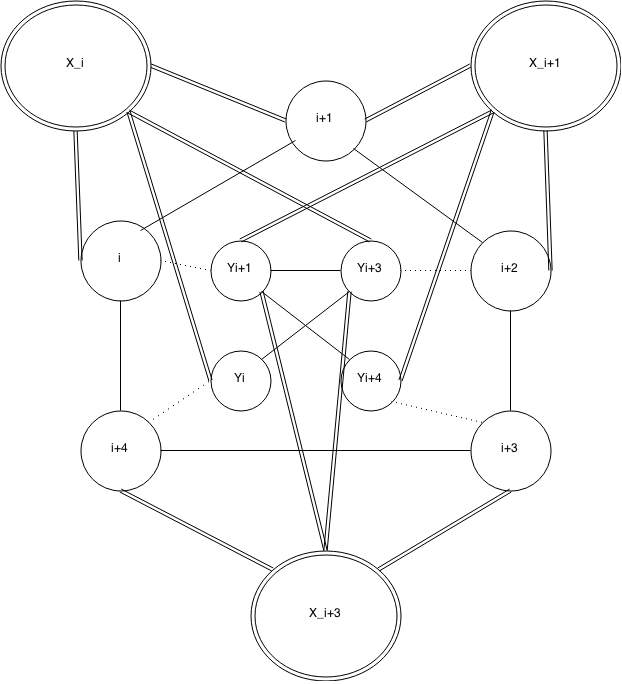
\includegraphics[width=\linewidth]{Base.png}
\end{minipage}

\begin{Observation}\label{obs:yi1-yi3-yi4} 
$|Y_{i+1}| = |Y_{i+3}| =  |Y_{i+4}| = 1$ and $|Y_{i}| = 0$
\end{Observation}

\begin{minipage}{0.5\textwidth}% adapt widths of minipages to your needs
	\noindent {\it Proof.} By Lemmas \ref{lem:yi-cojoins-yi1} and \ref{lem:yi-joins-yi2} $\chi(Y) = 2$. There are two cases to examine.
	\begin{itemize}
	\item[(i)]
		$|X_i| \leq |X_{i+1}|$ or $|X_{i+3}| \leq |X_{i+1}$

		 By Observation \ref{obs:xi-joins-yi} $\omega(G - Y) = \omega(G) - 2$. Since $\omega(G - Y) = \omega(G) - 2$ and $\chi(Y) = 2$ then by Observation \ref{obs:clique-chi} $\chi(G) = \omega(G)$.
	\item[(ii)]
		$|X_i| > |X_{i+1}$ and $|X_{i+3}| > |X_{i+1}|$

		By Observation \ref{obs:xi-joins-yi} $\omega(G - Y) = \omega(G) - 1$. $|X_{i+1}| + 2 + 1 = \omega(G) (X_{i+1},i+1,i+2, y_{i+3})$. By Observation \ref{obs:xj-g} both $X_{i+1} \cup X_{i+3}$ can be colored using $|X_{i}| - 1$ colors with a reserve color $k$ from $X_{i}$. Vertices $i+2 \cup i+4$ can use color $k$, vertex $i+3$ can share color with $i+1$, vertex $y_{i+4}$ can share a color with $y_{i+3}$ by Lemma \ref{yi-cojoins-yi1} , and vertex $y_{i+1}$ can share a color with $i$.  Then $\chi(G) = \omega(G)$.
	\end{itemize}
\end{minipage}
\hfill
\begin{minipage}{0.5\textwidth}\raggedleft
	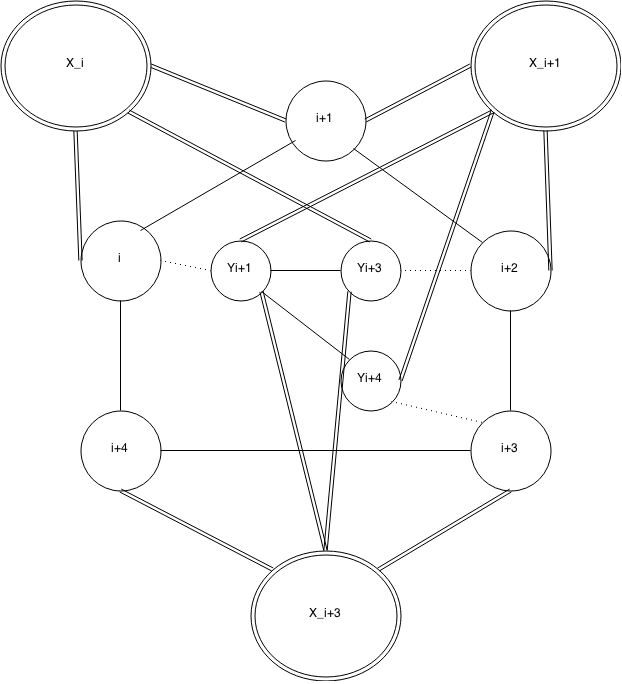
\includegraphics[width=\linewidth]{Yi1-Yi3-Yi4.png}
\end{minipage}



\begin{Observation}\label{obs:yi-yi1-yi3} 
$ |Y_{i}| = |Y_{i+1}| = |Y_{i+3}| = 1$ and $|Y_{i+4}| = 0$
\end{Observation}
\begin{minipage}{0.5\textwidth}% adapt widths of minipages to your needs
	\noindent {\it Proof.} By symmetry this case is equivalent to Case \ref{obs:yi1-yi3-yi4}.
\end{minipage}
\hfill
\begin{minipage}{0.5\textwidth}\raggedleft
	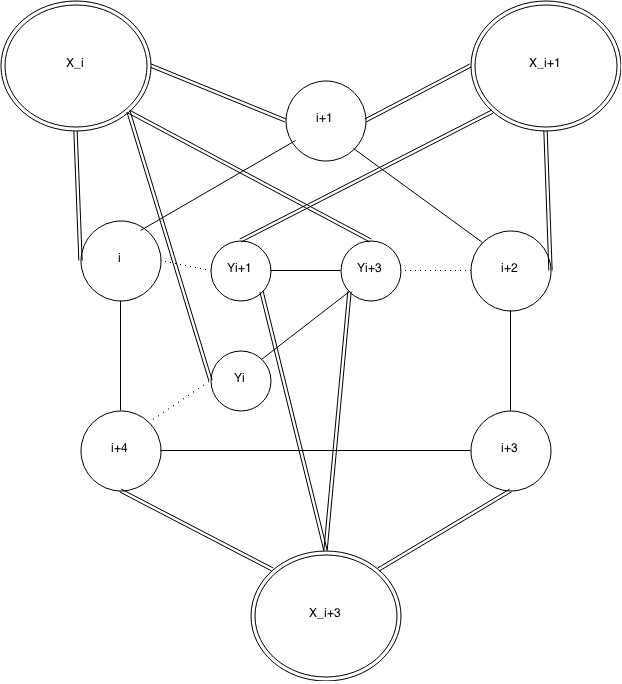
\includegraphics[width=\linewidth]{Yi-Yi1-Yi3.png}
\end{minipage}


\begin{Observation}\label{obs:yi-yi3-yi4} 
$|Y_{i}| = |Y_{i+3}| = |Y_{i+4}| = 1$ and $|Y_{i+1}| = 0$
\end{Observation} 
\begin{minipage}{0.5\textwidth}% adapt widths of minipages to your needs
	By Lemmas \ref{lem:yi-cojoins-yi1} and \ref{lem:yi-joins-yi2} $\chi(Y) = 2$. There are three cases to examine
	\begin{itemize}
	\item[(i)]
		$|X_i| \geq |X_{i+1}|$ and $|X_i| \geq |X_{i+3}|$.

		$\omega(G - Y) = \omega(G) - 2$ and $\chi(G) = \omega(G)$
	\item[(ii)]
		$|X_i| < |X_{i+3}| \leq |X_{i+1}$

		$\omega(G - Y) = \omega(G) - 1$. $|X_{i+1}| + 2 + 1 = \omega(G) (X_{i+1}, i+1, i+2, y_{i+4})$. A vertex $a \in X_i$ and a vertex $b \in X_{i+3}$ can share a color with $y_{i+4}$. By Observation \ref{obs:xj-uses-xi-one} and that $b \in |X_{i+3}|$ was colored then $X_{i} \cup X_{i+3}$ can be colored with $|X_{i+1}| -1$ colors leaving a color $k$ available from $X_{i+1}$. Vertex $i+3$ can share a color with $i+1$, vertex $i$ can share a color with $i+2$. Vertices $i+4$ and $y_{i}$ can use color $k$ since $y_{i} \cup i+4 \; \circled{0} X_i$ and $y_{i}i+4 \not \in E$. Then $G$ was colored with $\omega(G)$ colors.

	\item[(iii)]
		$|X_i| < |X_{i+1}| < |X_{i+3}$

		$\omega(G - Y) = \omega(G) - 1$. $|X_{i+3} + 2 + 1 = \omega(G) (X_{i+3}, i+3, i+4, y_{i+3})$. By Observation \ref{obs:xj-uses-xi-one} $X_i \cup X_{i+1}$ can be colored using $|X_{i+3}| -1 $ colors leaving a color $k$ available from $X_{i+3}$. Vertex $y_{i+4}$ can share a color with $y_{i+3}$, vertex $y_i$ can share a color with $i+4$, vertex $i+1$ can share a color with $i+3$, and vertices $i \cup i+2$ can use color $k$. Then $G$ was colored with $\omega(G)$ colors. 
	\end{itemize}
\end{minipage}
\hfill
\begin{minipage}{0.5\textwidth}\raggedleft
	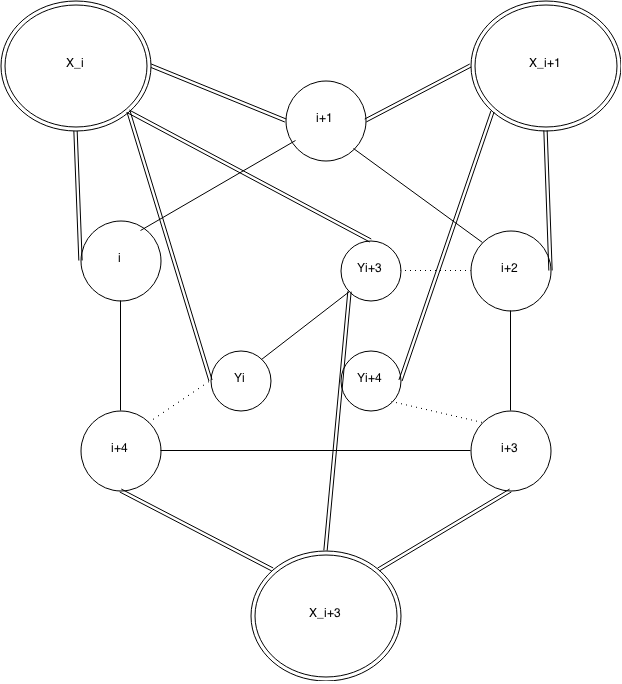
\includegraphics[width=\linewidth]{Yi-Yi3-Yi4.png}
\end{minipage}


\begin{Observation}\label{obs:yi-yi1-yi4} 
$|Y_{i}| = |Y_{i+1}| = |Y_{i+4}| = 1$ and $|Y_{i+3}| = 0$
\end{Observation}

\begin{minipage}{0.5\textwidth}% adapt widths of minipages to your needs
	\noindent {\it Proof.} By symmetry this case is equivalent to Case \ref{obs:yi-yi3-yi4}.
\end{minipage}
\hfill
\begin{minipage}{0.5\textwidth}\raggedleft
	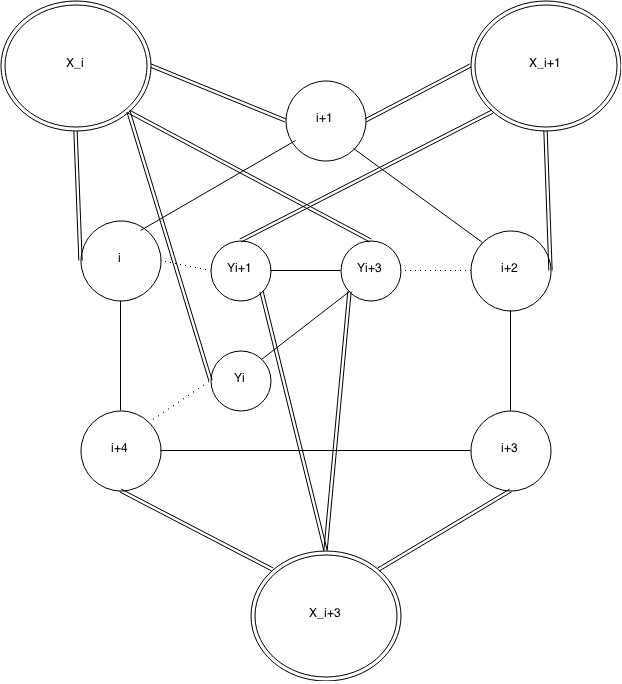
\includegraphics[width=\linewidth]{Yi-Yi1-Yi3.png}
\end{minipage}


\begin{Observation}\label{obs:yi1-yi4} 
$|Y_{i+1}| = |Y_{i+4}| = 1$ and $|Y_{i}| = |Y_{i+3}| = 0$
\end{Observation}

\begin{minipage}{0.5\textwidth}% adapt widths of minipages to your needs
	\noindent {\it Proof.} There are Four cases to examine.
	\begin{itemize}
	\item[(i)]
		$|X_{i+1}| \geq |X_i| \geq |X_{i+3}|$

		$\omega(G - Y) = \omega(G) - 2$ and $\chi(G) = \omega(G)$.

	\item[(ii)]
		$|X_{i+1}| \geq |X_i| - 1 \geq |X_{i+3}|$

		$\omega(G - Y) = \omega(G) - 1$. $|X_{i+1} + 2 + 1 = \omega(G) (X_{i+1}, i+1, i+2, y_{i+4})$. A vertex $\in X_i$ and a vertex $\in X_{i+3}$ can share a color with $y_{i+4}$. By Observation \ref{obs:xi-g-xj-g-xl} $X_i \cup X_{i+3}$ can be colored with $|X_{i+1}|$ colors with $X_{i+3}$ being colored with $|X_{i+1}| -1 $ colors leaving a color $k$. Vertex $i$ can use color $k$, vertex $i+2$ can share a color with $i+2$ and vertex $i+3$ can share a color with $i+1$. Then $G$ was colored with $\omega(G)$ colors.

	\item[(iii)]
		$|X_{i+3} \geq |X_{i}| > X_{i+1}$

		$\omega(G - Y) = \omega(G) - 1$. $|X_{i+3}| + 2 +1 = \omega(G) (X_{i+3}, i+3, i+4, y_{i+1})$. Vertices $y_{i+4}$ and $x_i \in X_i$ can share a color with $i+3$. $X_{i} \cup X_{i+1}$ can be colored using $|X_{i+3}|$ with a reserve color $k$ from $X_{i+3}$ since $|X_{i+3}| > |X_{i+1}|$ and $|X_{i+3}| > |X_i| - 1$. Vertex $i$ can share a color with $y_{i+1}$, vertex $i+1$ can share a color with $i+4$ and vertex $i+2$ use color $k$. Then $G$ was colored with $\omega(G)$ colors.

	\item[(iv)]
		$|X_{i}| > |X_{i+1}| - 1 \geq |X_{i+3}|$

		$\omega(G - Y) = \omega(G)$. $|X_{i} +2 = \omega(G) (X_{i}, i, i+1)$. By Observation \ref{obs:xi-g-xj-g-xl} $X_i|$ can be colored with $|X_i| - 1$ colors leaving a reserve color $k$ from $X_{i}$. By Observation \ref{obs:xi-g-xj-g-xl} $|X_{i+1}|$ can be colored with $|X_i| -2 $ colors leave reserve colors $k$ and $k_2$ from $X_{i}$. Vertex $y_{i+1}$ can share a color with $i$, vertex $y_{i+4}$ can use color $k_2$, vertices $y_{i+4} \cup i+3$ can use color $k$, vertex $i+2$ can use color $k_2$ and vertex $i+4$ can share a color with $i+1$. Then $G$ was colored with $\omega(G)$ colors.
	\end{itemize}
\end{minipage}
\hfill
\begin{minipage}{0.5\textwidth}\raggedleft
	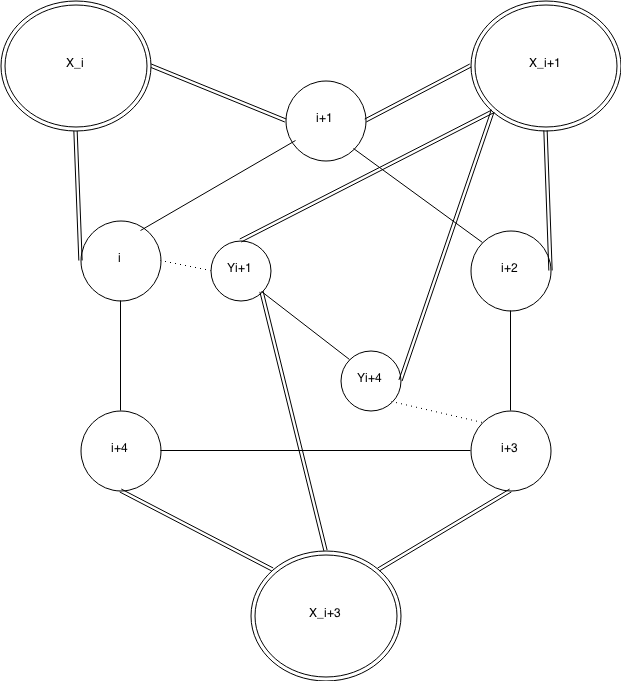
\includegraphics[width=\linewidth]{Yi1-Yi4.png}
\end{minipage}



\begin{Observation}\label{obs:yi-yi3} 
$|Y_{i}| = |Y_{i+3}| = 1$ and $|Y_{i+1}| = |Y_{i+4}| = 0$
\end{Observation}

\begin{minipage}{0.5\textwidth}% adapt widths of minipages to your needs
	\noindent {\it Proof.} By symmetry this case is equivalent to Case \ref{obs:yi1-yi4}
\end{minipage}
\hfill
\begin{minipage}{0.5\textwidth}\raggedleft
	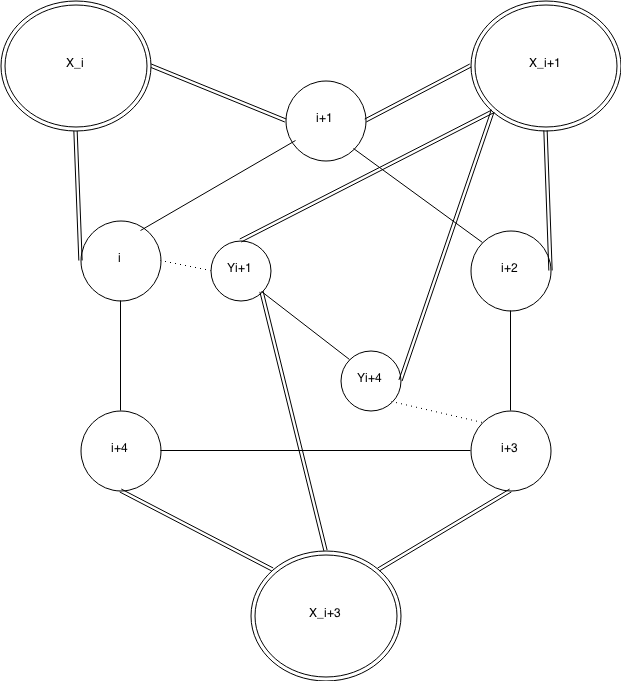
\includegraphics[width=\linewidth]{Yi-Yi3.png}
\end{minipage}


\begin{Observation}\label{obs:yi-yi4}
$|Y_{i}| = |Y_{i+4}| = 1$ and $|Y_{i+1}| = |Y_{i+3}| = 0$
\end{Observation}

\begin{minipage}{0.5\textwidth}% adapt widths of minipages to your needs
	\noindent {\it Proof.} There are two cases to examine
	\begin{itemize}
	\item[(i)]
	$|X_{i}| \geq  |X_{i+1}| \geq |X_{i+3}|$

	$\omega(G - Y) = \omega(G) - 1$. $y_i$ and $y_{i+4}$ can share a color hence $\varphi(G - Y) = \varphi(G) - 1$. By symmetry $|X_{i+1}| \geq  |X_{i}| \geq |X_{i+3}|$ is the same case.

	\item[(ii)]
	$|X_{i+3}| > |X_{i}| \geq |X_{i+1}|$

	$\omega(G - Y) = \omega(G)$. $|X_{i+3} +2 =\omega(G) (X_{i+3}, i+3, i+4$ By Observation \ref{obs:xi-g-xj-g-xl} $i+3$ can share colors with $y_{i+4}$ and a vertex $\in X_i$ and $i+4$ can share colors with $y_i$ and a vertex $\in X_{i+1}$. By Observation \ref{obs:xi-g-xj-g-xl} $X_i \cup X_{i+1}$ can be colored using at most $|X_{i+3} - 2$ since one vertex $\in X_i \cup X_{i+1}$ was already colored, reserving colors $k$ and $k_2$ from $X_{i+3}$. Vertices $i \cup i+2$ can use color $k$ and vertex $i+2$ can use color $k_2$. Then $G$ was colored with $\omega(G)$ colors.
	\end{itemize}
\end{minipage}
\hfill
\begin{minipage}{0.5\textwidth}\raggedleft
	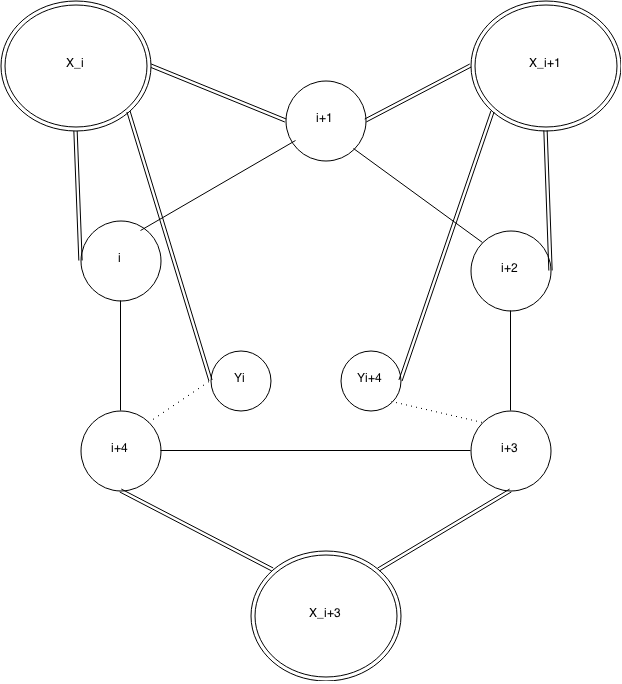
\includegraphics[width=\linewidth]{Yi-Yi4.png}
\end{minipage}


\begin{Observation}\label{obs:yi-yi1}
$|Y_{i}| = |Y_{i+1}| = 1$ and $|Y_{i+3}| = |Y_{i+4}| = 0$
\end{Observation}

\begin{minipage}{0.5\textwidth}% adapt widths of minipages to your needs
	\noindent {\it Proof.} There is only one cases to examine since $\omega(G - Y) = \omega(G) - 1 $. $y_{i} \cup y_{i+4}$ can share a color hence $\varphi(G - Y) = \varphi(G) - 1$.
\end{minipage}
\hfill
\begin{minipage}{0.5\textwidth}\raggedleft
	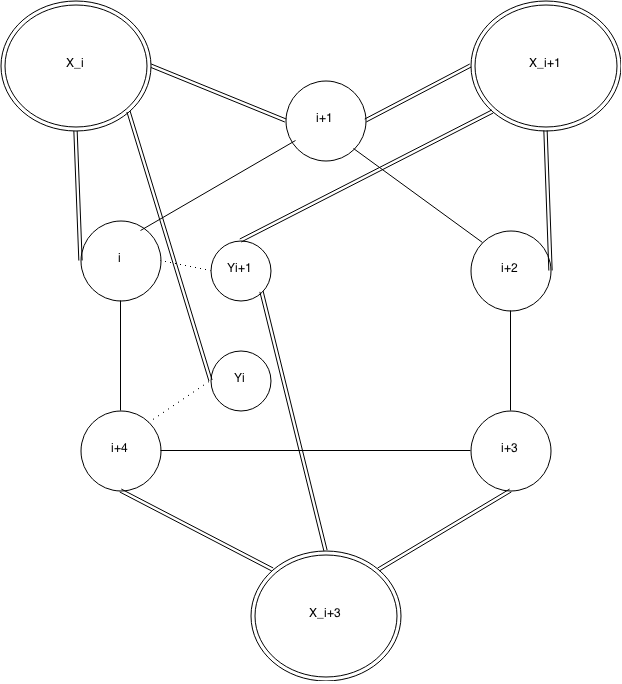
\includegraphics[width=\linewidth]{Yi-Yi1.png}
\end{minipage}



\begin{Observation}\label{obs:yi3-yi4}
$|Y_{i+3}| = |Y_{i+4}| = 1$ and $|Y_{i}| = |Y_{i+1}| = 0$
\end{Observation}

\begin{minipage}{0.5\textwidth}% adapt widths of minipages to your needs
	\noindent {\it Proof.} There are is only one cases to examine since $\omega(G - Y) = \omega(G) - 1 $. $y_{i} \cup y_{i+4}$ can share a color hence $\varphi(G - Y) = \varphi(G) - 1$.
\end{minipage}
\hfill
\begin{minipage}{0.5\textwidth}\raggedleft
	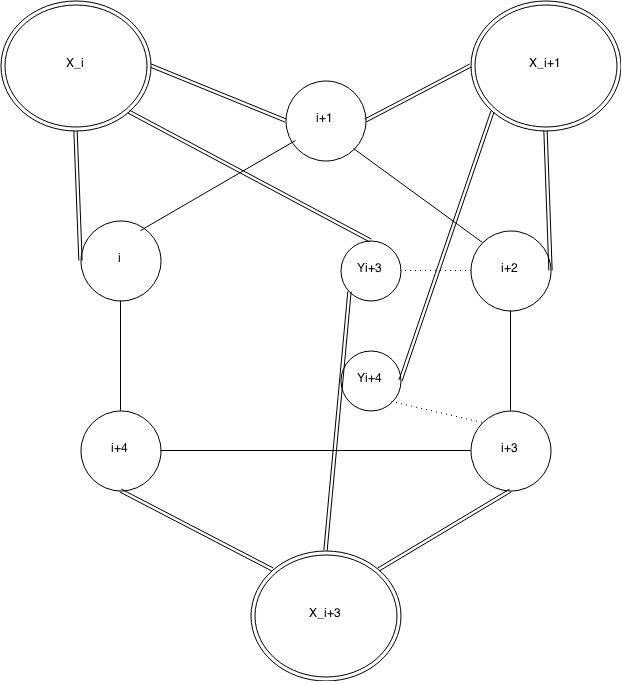
\includegraphics[width=\linewidth]{Yi3-Yi4.png}
\end{minipage}

\begin{Observation}\label{obs:yi1}
$|Y_{i+1}| = 1$ and $|Y_i| = |Y_{i+3}| = |Y_{i+4}| = 0$
\end{Observation}
\begin{minipage}{0.5\textwidth}% adapt widths of minipages to your needs
	\noindent {\it Proof} There are two cases to examine

	\begin{itemize}
	\item[(i)]
		$|X_i| \geq |X_{i+3}| \geq |X_{i+1}|$

		$\omega(G - Y) = \omega(G) - 1$. $y_{i+1}$ can use the new color and hence $\varphi(G) = \omega(G)$. The same argument can be made for $|X_{i+3}| \geq |X_i| \geq |X_{i+1}|$ 

	\item[(ii)]
		$|X_{i+1}| > |X_i| \geq |X_{i+3}|$

		$\omega(G - Y) = \omega(G)$. $|X_{i+1}| +2 = \omega(G) (X_{i+1}, i+1,i+2)$. By Observation \ref{obs:xi-g-xj-g-xl} $X_{i} \cup X_{i+3}$ can be colored with $|X_{i+1}|$ colors reserving color $k$ from $X_{i+1}$. Vertex $y_i$ can be share a color with $i$, vertex $i+3$ can share a color with $i+1$ and vertices $i+2 \cup i+4$ can use color $k$. Then $G$ was colored with $\omega(G)$ colors.
	\end{itemize}
\end{minipage}
\hfill
\begin{minipage}{0.5\textwidth}\raggedleft
	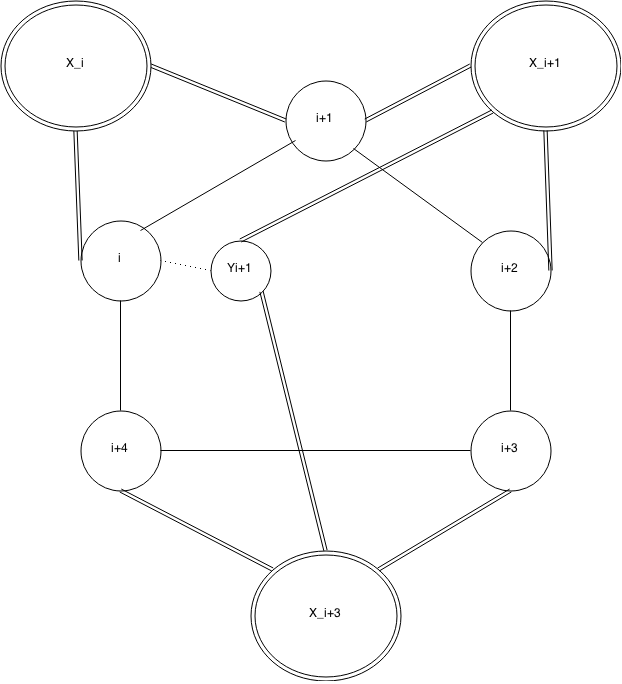
\includegraphics[width=\linewidth]{Yi1.png}
\end{minipage}


\begin{Observation}\label{obs:yi3}
$|Y_{i+3}| = 1$ and $|Y_i| = |Y_{i+1}| = |Y_{i+4}| = 0$
\end{Observation}

\begin{minipage}{0.5\textwidth}% adapt widths of minipages to your needs
	\noindent {\it Proof.} By symmetry this case is equivalent to \ref{obs:yi1}.
\end{minipage}
\hfill
\begin{minipage}{0.5\textwidth}\raggedleft
	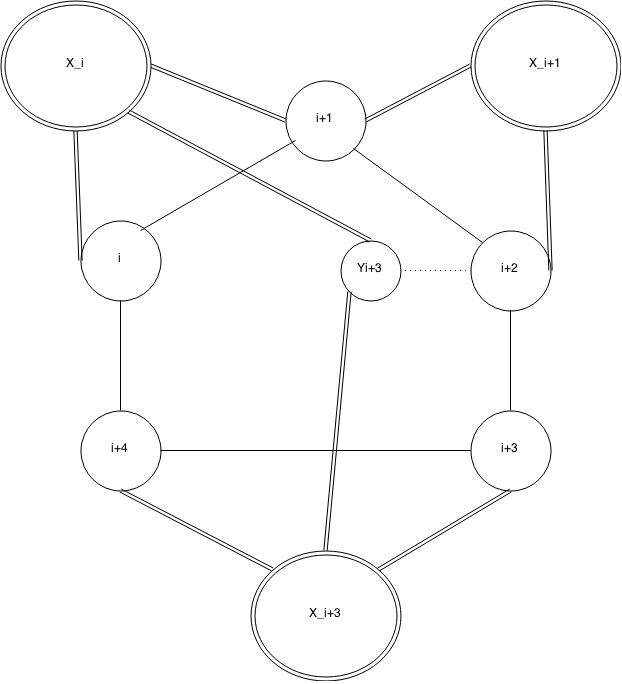
\includegraphics[width=\linewidth]{Yi3.png}
\end{minipage}



\begin{Observation}\label{obs:yi}
$|Y_{i}| = 1$ and $|Y_{i+1}| = |Y_{i+3}| = |Y_{i+4}| = 0$
\end{Observation}

\begin{minipage}{0.5\textwidth}% adapt widths of minipages to your needs
	\noindent {\it Proof} There are three cases to examine
	\begin{itemize}
		\item[(i)]
			$|X_{i+1}| \geq |X_i| \geq |X_{i+3}|$

			$\omega(G - Y) = \omega(G) - 1$. $y_{i}$ can use the new color and hence $\varphi(G) = \omega(G)$. 
		\item[(ii)]
			$|X_{i}| \geq |X_{i+3}| > |X_{i+1}|$
		
			$\omega(G - Y) = \omega(G)$. $|X_i| + 2 = \omega(G) (X_i, i, i+1)$. $X_{i+3}$ can be colored with $|X_i|$ colors and $X_{i+1}$ can be colored with $|X_i| - 1$ colors reserving a color $k$ from $X_i$. Vertex $i+2$ can share a color with $i$, vertex $i+4$ can share a color with $i+1$, and vertices $y_{i+4} \cup i+3$ can use color $k$.  Then $G$ was colroed with $\omega(G)$ colors.
		\item[(iii)]
			$|X_{i+3}| > |X_{i+1}| \geq |X_{i}|$.

			$\omega(G - Y) = \omega(G)$. $|X_{i+3} + 2 =\omega(G) (X_{i+3}, i+3, i+4)$. Vertex $y_{i+4}$ and a vertex $\in X_i$ can share a color with $i+3$. By Observation \ref{obs:xi-g-xj-g-xl} $X_{i+1} \cup X_{i}$ can be colored with $|X_{i+3}| - 1$ colors reserving color $k$ from $X_{i+3}$. Vertex $i+1$ can share a color with $i+4$, and vertices $i \cup i+2$ can share a color with $k$. Then $G$ was colored with $\omega(G)$ colors. 
	\end{itemize}
\end{minipage}
\hfill
\begin{minipage}{0.5\textwidth}\raggedleft
	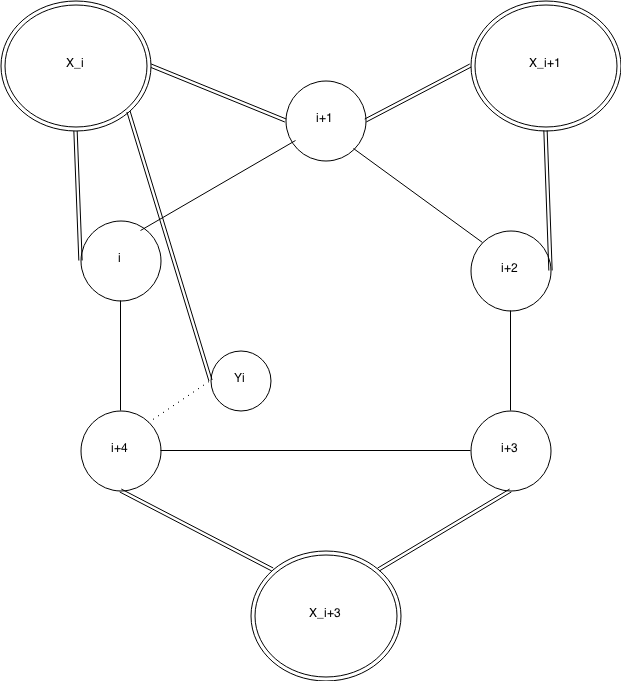
\includegraphics[width=\linewidth]{Yi.png}
\end{minipage}

\begin{Observation}\label{obs:yi4}
$|Y_{i+4}| = 1$ and $|Y_{i}| = |Y_{i+1}| = |Y_{i+3}| = 0$
\end{Observation}
\begin{minipage}{0.5\textwidth}% adapt widths of minipages to your needs
	\noindent {\it Proof.} By symmetry this case is equivalent to \ref{obs:yi}.
\end{minipage}
\hfill
\begin{minipage}{0.5\textwidth}\raggedleft
	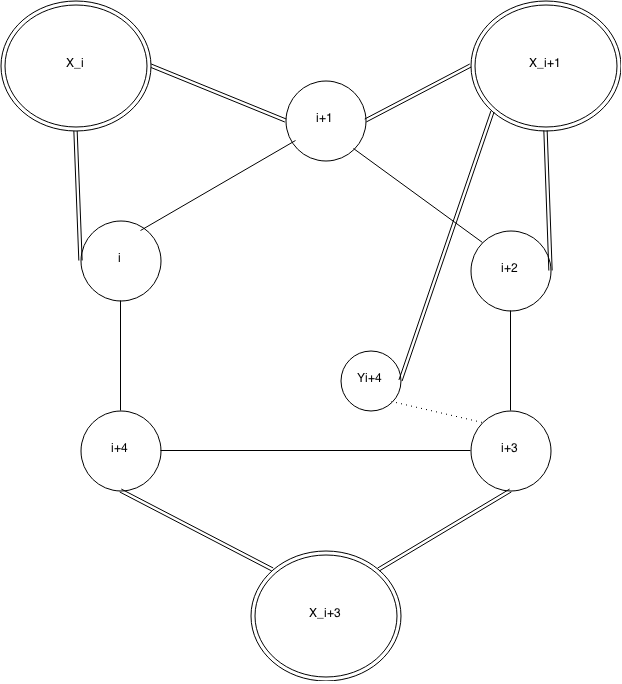
\includegraphics[width=\linewidth]{Yi4.png}
\end{minipage}

\begin{center}
{\bf Acknowledgement}
\end{center}
This work was done by authors  Laurier University. The authors A.M.H. and C.T.H. were each supported by individual NSERC Discovery Grants. D.J.F was supported by an NSERC Undergraduate Student Research Award.


\clearpage
\begin{thebibliography}{99}

\end{thebibliography}

\end{document}
